% Options for packages loaded elsewhere
\PassOptionsToPackage{unicode}{hyperref}
\PassOptionsToPackage{hyphens}{url}
%
\documentclass[
  man,floatsintext]{apa7}
\usepackage{amsmath,amssymb}
\usepackage{iftex}
\ifPDFTeX
  \usepackage[T1]{fontenc}
  \usepackage[utf8]{inputenc}
  \usepackage{textcomp} % provide euro and other symbols
\else % if luatex or xetex
  \usepackage{unicode-math} % this also loads fontspec
  \defaultfontfeatures{Scale=MatchLowercase}
  \defaultfontfeatures[\rmfamily]{Ligatures=TeX,Scale=1}
\fi
\usepackage{lmodern}
\ifPDFTeX\else
  % xetex/luatex font selection
\fi
% Use upquote if available, for straight quotes in verbatim environments
\IfFileExists{upquote.sty}{\usepackage{upquote}}{}
\IfFileExists{microtype.sty}{% use microtype if available
  \usepackage[]{microtype}
  \UseMicrotypeSet[protrusion]{basicmath} % disable protrusion for tt fonts
}{}
\makeatletter
\@ifundefined{KOMAClassName}{% if non-KOMA class
  \IfFileExists{parskip.sty}{%
    \usepackage{parskip}
  }{% else
    \setlength{\parindent}{0pt}
    \setlength{\parskip}{6pt plus 2pt minus 1pt}}
}{% if KOMA class
  \KOMAoptions{parskip=half}}
\makeatother
\usepackage{xcolor}
\usepackage{graphicx}
\makeatletter
\def\maxwidth{\ifdim\Gin@nat@width>\linewidth\linewidth\else\Gin@nat@width\fi}
\def\maxheight{\ifdim\Gin@nat@height>\textheight\textheight\else\Gin@nat@height\fi}
\makeatother
% Scale images if necessary, so that they will not overflow the page
% margins by default, and it is still possible to overwrite the defaults
% using explicit options in \includegraphics[width, height, ...]{}
\setkeys{Gin}{width=\maxwidth,height=\maxheight,keepaspectratio}
% Set default figure placement to htbp
\makeatletter
\def\fps@figure{htbp}
\makeatother
\setlength{\emergencystretch}{3em} % prevent overfull lines
\providecommand{\tightlist}{%
  \setlength{\itemsep}{0pt}\setlength{\parskip}{0pt}}
\setcounter{secnumdepth}{5}
% Make \paragraph and \subparagraph free-standing
\ifx\paragraph\undefined\else
  \let\oldparagraph\paragraph
  \renewcommand{\paragraph}[1]{\oldparagraph{#1}\mbox{}}
\fi
\ifx\subparagraph\undefined\else
  \let\oldsubparagraph\subparagraph
  \renewcommand{\subparagraph}[1]{\oldsubparagraph{#1}\mbox{}}
\fi
\newlength{\cslhangindent}
\setlength{\cslhangindent}{1.5em}
\newlength{\csllabelwidth}
\setlength{\csllabelwidth}{3em}
\newlength{\cslentryspacingunit} % times entry-spacing
\setlength{\cslentryspacingunit}{\parskip}
\newenvironment{CSLReferences}[2] % #1 hanging-ident, #2 entry spacing
 {% don't indent paragraphs
  \setlength{\parindent}{0pt}
  % turn on hanging indent if param 1 is 1
  \ifodd #1
  \let\oldpar\par
  \def\par{\hangindent=\cslhangindent\oldpar}
  \fi
  % set entry spacing
  \setlength{\parskip}{#2\cslentryspacingunit}
 }%
 {}
\usepackage{calc}
\newcommand{\CSLBlock}[1]{#1\hfill\break}
\newcommand{\CSLLeftMargin}[1]{\parbox[t]{\csllabelwidth}{#1}}
\newcommand{\CSLRightInline}[1]{\parbox[t]{\linewidth - \csllabelwidth}{#1}\break}
\newcommand{\CSLIndent}[1]{\hspace{\cslhangindent}#1}
\ifLuaTeX
\usepackage[bidi=basic]{babel}
\else
\usepackage[bidi=default]{babel}
\fi
\babelprovide[main,import]{english}
% get rid of language-specific shorthands (see #6817):
\let\LanguageShortHands\languageshorthands
\def\languageshorthands#1{}
% Manuscript styling
\usepackage{upgreek}
\captionsetup{font=singlespacing,justification=justified}

% Table formatting
\usepackage{longtable}
\usepackage{lscape}
% \usepackage[counterclockwise]{rotating}   % Landscape page setup for large tables
\usepackage{multirow}		% Table styling
\usepackage{tabularx}		% Control Column width
\usepackage[flushleft]{threeparttable}	% Allows for three part tables with a specified notes section
\usepackage{threeparttablex}            % Lets threeparttable work with longtable

% Create new environments so endfloat can handle them
% \newenvironment{ltable}
%   {\begin{landscape}\centering\begin{threeparttable}}
%   {\end{threeparttable}\end{landscape}}
\newenvironment{lltable}{\begin{landscape}\centering\begin{ThreePartTable}}{\end{ThreePartTable}\end{landscape}}

% Enables adjusting longtable caption width to table width
% Solution found at http://golatex.de/longtable-mit-caption-so-breit-wie-die-tabelle-t15767.html
\makeatletter
\newcommand\LastLTentrywidth{1em}
\newlength\longtablewidth
\setlength{\longtablewidth}{1in}
\newcommand{\getlongtablewidth}{\begingroup \ifcsname LT@\roman{LT@tables}\endcsname \global\longtablewidth=0pt \renewcommand{\LT@entry}[2]{\global\advance\longtablewidth by ##2\relax\gdef\LastLTentrywidth{##2}}\@nameuse{LT@\roman{LT@tables}} \fi \endgroup}

% \setlength{\parindent}{0.5in}
% \setlength{\parskip}{0pt plus 0pt minus 0pt}

% Overwrite redefinition of paragraph and subparagraph by the default LaTeX template
% See https://github.com/crsh/papaja/issues/292
\makeatletter
\renewcommand{\paragraph}{\@startsection{paragraph}{4}{\parindent}%
  {0\baselineskip \@plus 0.2ex \@minus 0.2ex}%
  {-1em}%
  {\normalfont\normalsize\bfseries\itshape\typesectitle}}

\renewcommand{\subparagraph}[1]{\@startsection{subparagraph}{5}{1em}%
  {0\baselineskip \@plus 0.2ex \@minus 0.2ex}%
  {-\z@\relax}%
  {\normalfont\normalsize\itshape\hspace{\parindent}{#1}\textit{\addperi}}{\relax}}
\makeatother

% \usepackage{etoolbox}
\makeatletter
\patchcmd{\HyOrg@maketitle}
  {\section{\normalfont\normalsize\abstractname}}
  {\section*{\normalfont\normalsize\abstractname}}
  {}{\typeout{Failed to patch abstract.}}
\patchcmd{\HyOrg@maketitle}
  {\section{\protect\normalfont{\@title}}}
  {\section*{\protect\normalfont{\@title}}}
  {}{\typeout{Failed to patch title.}}
\makeatother

\usepackage{xpatch}
\makeatletter
\xapptocmd\appendix
  {\xapptocmd\section
    {\addcontentsline{toc}{section}{\appendixname\ifoneappendix\else~\theappendix\fi\\: #1}}
    {}{\InnerPatchFailed}%
  }
{}{\PatchFailed}
\keywords{keywords}
\usepackage{csquotes}
\makeatletter
\renewcommand{\paragraph}{\@startsection{paragraph}{4}{\parindent}%
  {0\baselineskip \@plus 0.2ex \@minus 0.2ex}%
  {-1em}%
  {\normalfont\normalsize\bfseries\typesectitle}}

\renewcommand{\subparagraph}[1]{\@startsection{subparagraph}{5}{1em}%
  {0\baselineskip \@plus 0.2ex \@minus 0.2ex}%
  {-\z@\relax}%
  {\normalfont\normalsize\bfseries\itshape\hspace{\parindent}{#1}\textit{\addperi}}{\relax}}
\makeatother

\ifLuaTeX
  \usepackage{selnolig}  % disable illegal ligatures
\fi
\IfFileExists{bookmark.sty}{\usepackage{bookmark}}{\usepackage{hyperref}}
\IfFileExists{xurl.sty}{\usepackage{xurl}}{} % add URL line breaks if available
\urlstyle{same}
\hypersetup{
  pdftitle={A Diverse Happiness for a Diversifing World: The Relationship between Community-level Racial Diversity and Psycholoigcal Richness},
  pdfauthor={Brett Neely Peterson1 \& Ernst-August Doelle1,2},
  pdflang={en-EN},
  pdfkeywords={keywords},
  hidelinks,
  pdfcreator={LaTeX via pandoc}}

\title{A Diverse Happiness for a Diversifing World: The Relationship between Community-level Racial Diversity and Psycholoigcal Richness}
\author{Brett Neely Peterson\textsuperscript{1} \& Ernst-August Doelle\textsuperscript{1,2}}
\date{}


\shorttitle{A Diverse Happiness for a Diversifing World}

\authornote{

Please email \href{mailto:bnpeterson@uchicago.edu}{\nolinkurl{bnpeterson@uchicago.edu}} for questions about this important research.

The authors made the following contributions. Brett Neely Peterson: Conceptualization, Writing - Original Draft Preparation, Writing - Review \& Editing; Ernst-August Doelle: Writing - Review \& Editing, Supervision.

Correspondence concerning this article should be addressed to Brett Neely Peterson, Postal address. E-mail: \href{mailto:bnpeterson@uchicago.edu}{\nolinkurl{bnpeterson@uchicago.edu}}

}

\affiliation{\vspace{0.5cm}\textsuperscript{1} The University of Chicago}

\abstract{%
One or two sentences providing a \textbf{basic introduction} to the field, comprehensible to a scientist in any discipline.
}



\begin{document}
\maketitle

\hypertarget{literature-review}{%
\section{Literature Review}\label{literature-review}}

\hypertarget{a-diversifying-world}{%
\subsection{A Diversifying World}\label{a-diversifying-world}}

Increasing levels of diversity have become hallmarks of the modern, globalizing world. With greater global inter-connectivity, the expanded communication tools, technological development, and the increased global migration, many people now have greater opportunities to interact with people different from themselves racially, religious, or culturally than perhaps at any other point in history. This increasing diversification presents both profound possibilities and potential challenges as people grapple with the changing social and communal dynamics. Therefore, in light of both this increasing diversification and the often mixed responses to it, it is especially valuable now to understand how living within a diverse community impacts individual well-being. However, the relationship between diversity and psychological richness, a vital component of human well-being, has largely gone unexplored up to this point. Therefore, this paper will seek to address this question of how living within a racially diverse community affects individual levels of psychological richness through a series of studies in this area. In order to address this question, this paper proposes a two primary hypotheses regarding the relationship between the degree of diversity in one's community and the prevalence of psychological richness:

\begin{quote}
\emph{H1: Living within an ethnically diverse or heterogeneous community leads people to have greater degrees of psychological richness.}
\end{quote}

\begin{quote}
\emph{H2: This change in psychological richness is at least partially explained by a more racially diverse social networks exposing individuals to different perspectives and experiences.}
\end{quote}

In order to address this central question regarding diversity and psychological richness along with these corresponding hypotheses, however, one must first examine the current relevant literature regarding diversity, well-being, and psychological richness so that a clear link between these concepts can be established.

\hypertarget{constrict-theory-a-direct-challenge-to-well-being}{%
\subsection{Constrict Theory: A Direct Challenge to Well-being}\label{constrict-theory-a-direct-challenge-to-well-being}}

First, understanding the impact of diversity on the different members within a community is vital for understanding how it might impact individual well-being. In his landmark research findings on diversity,
Putnam (2007) finally addressed the on-going debate between the contact and conflict theories of diversity by presenting extensive data supporting a new model, known as the ``constrict theory'' of social capital (p.~144). Rather than either decreasing racial animosity (Allport, 1954; Brown et al., 2021; Du Bois, 1899; Sigelman \& Welch, 1993; Stouffer et al., 1949) or increasing a sense of outgroup threat (Enos, 2014, 2016; Giles \& Evans, 1986; Herbert Blumer, 1958), Putnam found that diversity actually has this ``constricting'' effect where increasing diversity actually lowers trust for both in-group and out-group communities which leads to greater social isolation and overall weaker social capital (Putnam, 2007, pp. 144, 149--150). Based on Putnam's research regarding the constrict theory, therefore, one could reasonably assume that greater diversity may lead to lower overall well-being since happiness and meaning, two of the primary factors in well-being, are both connected to social support and connecting to something greater than one's self (Oishi \& Westgate, 2022, pp. 791--792). In fact, Seder and Oishi (2009) actually found this type of diversity effect when conducting research that demonstrated university students with more homogenous friendship networks on Facebook actually scored higher on life satisfaction and positive feelings than those with more heterogenous networks (p.~443). Similar results were also found both by Florez et al. (2019) who demonstrated that higher levels of meaning are associated with higher degrees of prejudice and by Elnakouri et al. (2022, p. 5) who demonstrated that collective hate towards a group, as opposed to individual hate towards a specific person often produced higher meaning in life. Therefore, based on the preponderance of the current research on diversity and its impact on well-being, one might reasonably assume that living within a diverse community would reduce overall well-being.

\hypertarget{a-potential-answer-psychological-richness}{%
\subsection{A Potential Answer: Psychological Richness}\label{a-potential-answer-psychological-richness}}

While portions of the current literature may appear to present a negative view of diversity at first glance, however, there are also substantive reasons to believe that this may not be the full picture. The current literature on diversity does convincingly demonstrate that increased diversity likely reduces happiness and meaning in certain circumstances, but these are not the only two factors that contribute to well-being. Oishi and Westgate provide compelling evidence that the current framework of human well-being should be expanded beyond happiness and meaning, to also include psychological richness, a third vital and distinct element of living a good life (Oishi \& Westgate, 2022, p. 790). While happiness is associated with stability and satisfaction, and meaning with a greater purpose, psychological richness on the other hand is defined by a sense of experiencing perspective-changing exploration that contributes to living a good life (Oishi \& Westgate, 2022, p. 790). In this manner, psychological richness is often associated with an openness to new experiences, an awareness that one's perspective is not definitive or universal, a higher penchant for creativity and narrative complexity, and also a willingness to consider challenging experiences rewarding even if difficult (Oishi \& Westgate, 2022, pp. 790, 794, 797--798, 804). Because of these different causes and features, it is possible that psychological richness may have a different relationship with diversity than either happiness or meaning. Therefore, since past studies have only focused on the relationship between diversity and these first two components of well-being, it also remains possible that the current literature on diversity has unintentionally presented an overly negative portrayal of diversity by not considering how it may impact psychological richness as well.

Additionally, there are reasons to believe that psychological richness, unlike happiness and meaning, is positively correlated with diversity based on the current literature. First, political liberalism, a factor commonly associated with racial openness, is instead highly related to psychological richness (Oishi et al., 2021, p. 755). Second, psychological richness has proven to be more resistant to challenges and traumatic events than either happiness or meaning, so it is possible that the different challenges inherent in increasing diversity may not affect psychological richness in the same way as its counterparts (Oishi \& Westgate, 2022, pp. 804--804). Finally, while a link between diversity and psychological richness has yet to be definitively proven, the current research has demonstrated that certain experiences which involve increased exposure to diversity, such as studying abroad, do in fact increase rates of psychological richness while not having a similar impact on happiness or meaning (Oishi \& Westgate, 2022, p. 797). Based on the substantive evidence of the current literature on psychological richness, therefore, there are substantial reasons to believe that psychological richness, unlike happiness and meaning, may actually have a positive causal relationship with increased racial diversity.

\hypertarget{methods}{%
\section{Methods}\label{methods}}

We report how we determined our sample size, all data exclusions (if any), all manipulations, and all measures in the study.

\hypertarget{participants}{%
\subsection{Participants}\label{participants}}

\hypertarget{material}{%
\subsection{Material}\label{material}}

\hypertarget{procedure}{%
\subsection{Procedure}\label{procedure}}

\begin{figure}
\centering
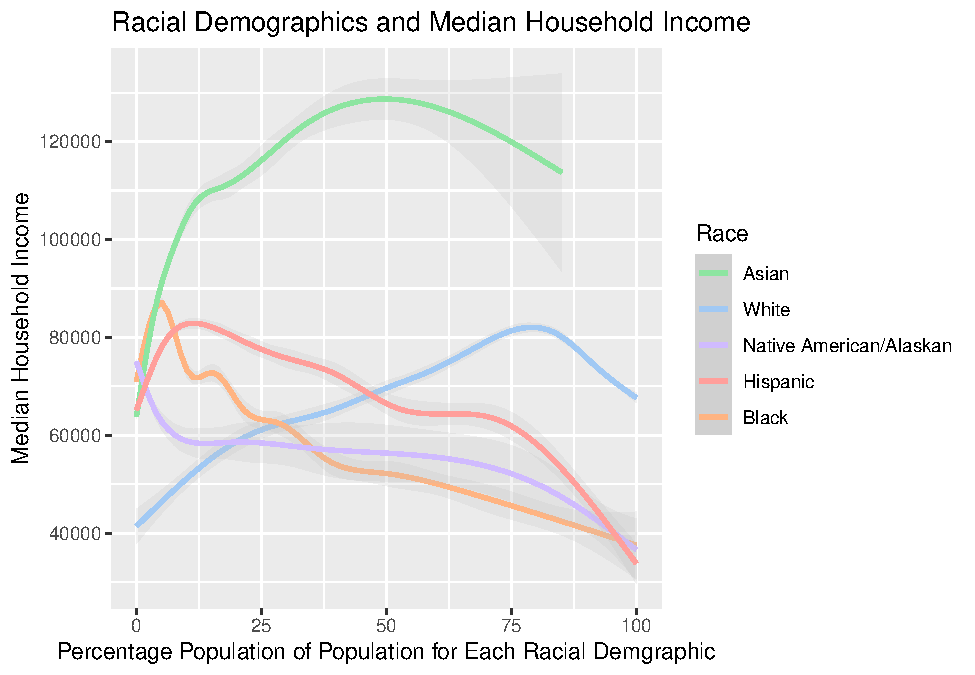
\includegraphics{ZIP-Diversity-Income-Markdown_files/figure-latex/race-median-income-smooth-fig-1.pdf}
\caption{\label{fig:race-median-income-smooth-fig}ZIP Code Median Household Income by Percentage of the Poluation of Each Demgraphic}
\end{figure}

This is to check whether I can finally reference Figure \ref{fig:race-median-income-smooth-fig}.

\begin{figure}
\centering
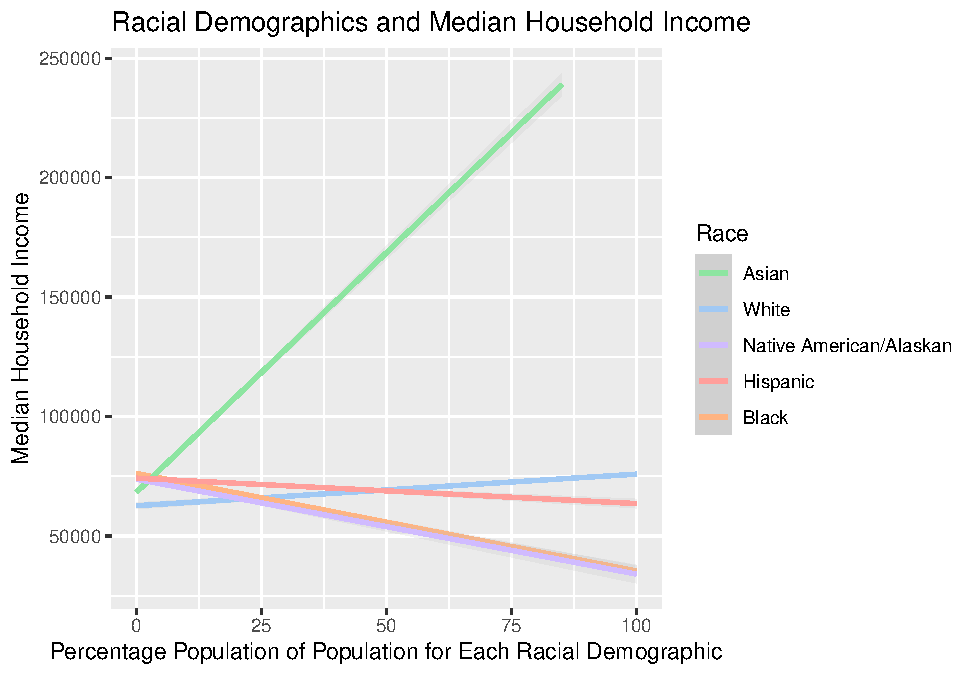
\includegraphics{ZIP-Diversity-Income-Markdown_files/figure-latex/race-median-income-lm-fig-1.pdf}
\caption{\label{fig:race-median-income-lm-fig}ZIP Code Median Household Income by Percentage of the Poluation of Each Demgraphic}
\end{figure}

This is to check whether I can finally reference Figure \ref{fig:race-median-income-lm-fig}.

\hypertarget{data-analysis}{%
\subsection{Data analysis}\label{data-analysis}}

In Model 1, which includes just one independent variable (\texttt{Median\_Household\_Income\ \textasciitilde{}\ X\_Total\_Population\_White\_Alone}), the percentage of the ZIP Code population that is white is positively associated with median household income (\(\beta\) = 132.29, \(p\) \textless{} 0.00). The Intercept, or approximated mean of median household income if the percent white were were zero, is \$62693.04, and for every additional unit of percent of the population white, we expect an increase of \$132.29. (Additionally, it is important to note that the Intercept is different than the mean median household income for all ZIP Codes \$73132.63.) Therefore, if we increased percent white by one unit that manner, we would expect the mean ZIP Code median household income to increase to \$62825.33. Additionally, Model 1 shows a very significant relationship between percent of the population white and median household income (\textless{} .001) indicating a strong association between the two variables.

We used R (Version 4.3.1; R Core Team, 2023) and the R-packages \emph{broom} (Version 1.0.5; Robinson et al., 2023), \emph{dplyr} (Version 1.1.4; Wickham, François, et al., 2023), \emph{forcats} (Version 1.0.0; Wickham, 2023a), \emph{ggplot2} (Version 3.4.3; Wickham, 2016), \emph{jtools} (Version 2.2.2; Long, 2022), \emph{lme4} (Version 1.1.35.1; Bates et al., 2015), \emph{lubridate} (Version 1.9.3; Grolemund \& Wickham, 2011), \emph{Matrix} (Version 1.6.1.1; Bates et al., 2023), \emph{papaja} (Version 0.1.1.9001; Aust \& Barth, 2023), \emph{psych} (Version 2.4.1; William Revelle, 2024), \emph{purrr} (Version 1.0.2; Wickham \& Henry, 2023), \emph{readr} (Version 2.1.4; Wickham, Hester, et al., 2023), \emph{readxl} (Version 1.4.3; Wickham \& Bryan, 2023), \emph{scales} (Version 1.3.0; Wickham, Pedersen, et al., 2023), \emph{shiny} (Version 1.8.0; Chang et al., 2023), \emph{stringr} (Version 1.5.1; Wickham, 2023b), \emph{tibble} (Version 3.2.1; Müller \& Wickham, 2023), \emph{tidyr} (Version 1.3.1; Wickham, Vaughan, et al., 2023), \emph{tidyverse} (Version 2.0.0; Wickham et al., 2019), \emph{tinylabels} (Version 0.2.4; Barth, 2023), \emph{tinytex} (Version 0.49; Xie, 2019), and \emph{writexl} (Version 1.5.0; Ooms, 2024) for all our analyses.

\hypertarget{results}{%
\section{Results}\label{results}}

\hypertarget{discussion}{%
\section{Discussion}\label{discussion}}

\newpage

\hypertarget{references}{%
\section{References}\label{references}}

\hypertarget{refs}{}
\begin{CSLReferences}{1}{0}
\leavevmode\vadjust pre{\hypertarget{ref-allportNaturePrejudiceGordon1954}{}}%
Allport, G. W. (1897.-1967). A. (1954). \emph{The nature of prejudice / {Gordon W}. {Allport}}. {Addison-Wesley Publishing Company}.

\leavevmode\vadjust pre{\hypertarget{ref-R-papaja}{}}%
Aust, F., \& Barth, M. (2023). \emph{{papaja}: {Prepare} reproducible {APA} journal articles with {R Markdown}}. \url{https://github.com/crsh/papaja}

\leavevmode\vadjust pre{\hypertarget{ref-R-tinylabels}{}}%
Barth, M. (2023). \emph{{tinylabels}: Lightweight variable labels}. \url{https://cran.r-project.org/package=tinylabels}

\leavevmode\vadjust pre{\hypertarget{ref-R-lme4}{}}%
Bates, D., Mächler, M., Bolker, B., \& Walker, S. (2015). Fitting linear mixed-effects models using {lme4}. \emph{Journal of Statistical Software}, \emph{67}(1), 1--48. \url{https://doi.org/10.18637/jss.v067.i01}

\leavevmode\vadjust pre{\hypertarget{ref-R-Matrix}{}}%
Bates, D., Maechler, M., \& Jagan, M. (2023). \emph{Matrix: Sparse and dense matrix classes and methods}. \url{https://CRAN.R-project.org/package=Matrix}

\leavevmode\vadjust pre{\hypertarget{ref-brownChildhoodCrossethnicExposure2021}{}}%
Brown, J. r., Enos, R. d., Mazumder, S., \& Feigenbaum, J. (2021). Childhood cross-ethnic exposure predicts political behavior seven decades later: {Evidence} from linked administrative data. \emph{Science Advances}, \emph{7}(24). \url{https://doi.org/10.1126/sciadv.abe8432}

\leavevmode\vadjust pre{\hypertarget{ref-R-shiny}{}}%
Chang, W., Cheng, J., Allaire, J., Sievert, C., Schloerke, B., Xie, Y., Allen, J., McPherson, J., Dipert, A., \& Borges, B. (2023). \emph{Shiny: Web application framework for r}. \url{https://CRAN.R-project.org/package=shiny}

\leavevmode\vadjust pre{\hypertarget{ref-duboisPhiladelphiaNegroSocial1899}{}}%
Du Bois, W. E. B. (1899). \emph{The {Philadelphia Negro}: A social study}. {Published for the University}.

\leavevmode\vadjust pre{\hypertarget{ref-elnakouriHateMeaningLife2022a}{}}%
Elnakouri, A., Hubley, C., \& McGregor, I. (2022). Hate and meaning in life: {How} collective, but not personal, hate quells threat and spurs meaning in life. \emph{Journal of Experimental Social Psychology}, \emph{98}. \url{https://doi.org/10.1016/j.jesp.2021.104227}

\leavevmode\vadjust pre{\hypertarget{ref-enosCausalEffectIntergroup2014}{}}%
Enos, R. D. (2014). Causal effect of intergroup contact on exclusionary attitudes. \emph{Proceedings of the National Academy of Sciences of the United States of America}, \emph{111}(10), 3699--3704.

\leavevmode\vadjust pre{\hypertarget{ref-enosWhatDemolitionPublic2016}{}}%
Enos, R. D. (2016). What the {Demolition} of {Public Housing Teaches Us} about the {Impact} of {Racial Threat} on {Political Behavior}. \emph{American Journal of Political Science}, \emph{60}(1), 123--142.

\leavevmode\vadjust pre{\hypertarget{ref-florezUnderstandingMeaningRacial2019a}{}}%
Florez, I. A., Schulenberg, S. E., Lair, E. C., Wilson, K. G., \& Johnson, K. A. (2019). Understanding meaning and racial prejudice: {Examining} self-transcendence and psychological inflexibility in a sample of {White} college students. \emph{Journal of Contextual Behavioral Science}, \emph{12}, 1--6. \url{https://doi.org/10.1016/j.jcbs.2018.11.007}

\leavevmode\vadjust pre{\hypertarget{ref-gilesPowerApproachIntergroup1986}{}}%
Giles, M. W., \& Evans, A. (1986). The {Power Approach} to {Intergroup Hostility}. \emph{Journal of Conflict Resolution}, \emph{30}(3), 469--486. \url{https://doi.org/10.1177/0022002786030003004}

\leavevmode\vadjust pre{\hypertarget{ref-R-lubridate}{}}%
Grolemund, G., \& Wickham, H. (2011). Dates and times made easy with {lubridate}. \emph{Journal of Statistical Software}, \emph{40}(3), 1--25. \url{https://www.jstatsoft.org/v40/i03/}

\leavevmode\vadjust pre{\hypertarget{ref-herbertblumerRacePrejudiceSense1958}{}}%
Herbert Blumer. (1958). Race {Prejudice} as a {Sense} of {Group Position}. \emph{The Pacific Sociological Review}, \emph{1}, 3--7.

\leavevmode\vadjust pre{\hypertarget{ref-R-jtools}{}}%
Long, J. A. (2022). \emph{Jtools: Analysis and presentation of social scientific data}. \url{https://cran.r-project.org/package=jtools}

\leavevmode\vadjust pre{\hypertarget{ref-R-tibble}{}}%
Müller, K., \& Wickham, H. (2023). \emph{Tibble: Simple data frames}. \url{https://CRAN.R-project.org/package=tibble}

\leavevmode\vadjust pre{\hypertarget{ref-oishiExperiencesAssociatedPsychological2021}{}}%
Oishi, S., Choi, H., Liu, A., \& Kurtz, J. (2021). Experiences associated with psychological richness. \emph{European Journal of Personality}, \emph{35}(5), 754--770. \url{https://doi.org/10.1177/0890207020962334}

\leavevmode\vadjust pre{\hypertarget{ref-oishiPsychologicallyRichLife2022}{}}%
Oishi, S., \& Westgate, E. c. (2022). A {Psychologically Rich Life}: {Beyond Happiness} and {Meaning}. \emph{Psychological Review}, \emph{129}(4), 790--811. \url{https://doi.org/10.1037/rev0000317}

\leavevmode\vadjust pre{\hypertarget{ref-R-writexl}{}}%
Ooms, J. (2024). \emph{Writexl: Export data frames to excel 'xlsx' format}. \url{https://CRAN.R-project.org/package=writexl}

\leavevmode\vadjust pre{\hypertarget{ref-putnamPluribusUnumDiversity2007}{}}%
Putnam, R. D. (2007). E {Pluribus Unum}: {Diversity} and {Community} in the {Twenty-first Century The} 2006 {Johan Skytte Prize Lecture}. \emph{Scandinavian Political Studies}, \emph{30}(2), 137--174. \url{https://doi.org/10.1111/j.1467-9477.2007.00176.x}

\leavevmode\vadjust pre{\hypertarget{ref-R-base}{}}%
R Core Team. (2023). \emph{R: A language and environment for statistical computing}. R Foundation for Statistical Computing. \url{https://www.R-project.org/}

\leavevmode\vadjust pre{\hypertarget{ref-R-broom}{}}%
Robinson, D., Hayes, A., \& Couch, S. (2023). \emph{Broom: Convert statistical objects into tidy tibbles}. \url{https://CRAN.R-project.org/package=broom}

\leavevmode\vadjust pre{\hypertarget{ref-sederEthnicRacialHomogeneity2009e}{}}%
Seder, J. P., \& Oishi, S. (2009). Ethnic/racial homogeneity in college students' {Facebook} friendship networks and subjective well-being. \emph{Journal of Research in Personality}, \emph{43}(3), 438--443. \url{https://doi.org/10.1016/j.jrp.2009.01.009}

\leavevmode\vadjust pre{\hypertarget{ref-sigelmanContactHypothesisRevisited1993}{}}%
Sigelman, L., \& Welch, S. (1993). The contact hypothesis revisited: Black-white interaction and positive racial attitudes. \emph{Social Forces}, \emph{71}(3), 781--795. \url{https://doi.org/10.1093/sf/71.3.781}

\leavevmode\vadjust pre{\hypertarget{ref-stoufferAmericanSoldierAdjustment1949}{}}%
Stouffer, S. A., Suchman, E. A., Devinney, L. C., Star, S. A., \& Williams Jr., R. M. (1949). \emph{The {American} soldier: {Adjustment} during army life. ({Studies} in social psychology in {World War II}), {Vol}. 1} (pp. xii, 599). {Princeton Univ. Press}.

\leavevmode\vadjust pre{\hypertarget{ref-R-ggplot2}{}}%
Wickham, H. (2016). \emph{ggplot2: Elegant graphics for data analysis}. Springer-Verlag New York. \url{https://ggplot2.tidyverse.org}

\leavevmode\vadjust pre{\hypertarget{ref-R-forcats}{}}%
Wickham, H. (2023a). \emph{Forcats: Tools for working with categorical variables (factors)}. \url{https://CRAN.R-project.org/package=forcats}

\leavevmode\vadjust pre{\hypertarget{ref-R-stringr}{}}%
Wickham, H. (2023b). \emph{Stringr: Simple, consistent wrappers for common string operations}. \url{https://CRAN.R-project.org/package=stringr}

\leavevmode\vadjust pre{\hypertarget{ref-R-tidyverse}{}}%
Wickham, H., Averick, M., Bryan, J., Chang, W., McGowan, L. D., François, R., Grolemund, G., Hayes, A., Henry, L., Hester, J., Kuhn, M., Pedersen, T. L., Miller, E., Bache, S. M., Müller, K., Ooms, J., Robinson, D., Seidel, D. P., Spinu, V., \ldots{} Yutani, H. (2019). Welcome to the {tidyverse}. \emph{Journal of Open Source Software}, \emph{4}(43), 1686. \url{https://doi.org/10.21105/joss.01686}

\leavevmode\vadjust pre{\hypertarget{ref-R-readxl}{}}%
Wickham, H., \& Bryan, J. (2023). \emph{Readxl: Read excel files}. \url{https://CRAN.R-project.org/package=readxl}

\leavevmode\vadjust pre{\hypertarget{ref-R-dplyr}{}}%
Wickham, H., François, R., Henry, L., Müller, K., \& Vaughan, D. (2023). \emph{Dplyr: A grammar of data manipulation}. \url{https://CRAN.R-project.org/package=dplyr}

\leavevmode\vadjust pre{\hypertarget{ref-R-purrr}{}}%
Wickham, H., \& Henry, L. (2023). \emph{Purrr: Functional programming tools}. \url{https://CRAN.R-project.org/package=purrr}

\leavevmode\vadjust pre{\hypertarget{ref-R-readr}{}}%
Wickham, H., Hester, J., \& Bryan, J. (2023). \emph{Readr: Read rectangular text data}. \url{https://CRAN.R-project.org/package=readr}

\leavevmode\vadjust pre{\hypertarget{ref-R-scales}{}}%
Wickham, H., Pedersen, T. L., \& Seidel, D. (2023). \emph{Scales: Scale functions for visualization}. \url{https://CRAN.R-project.org/package=scales}

\leavevmode\vadjust pre{\hypertarget{ref-R-tidyr}{}}%
Wickham, H., Vaughan, D., \& Girlich, M. (2023). \emph{Tidyr: Tidy messy data}. \url{https://CRAN.R-project.org/package=tidyr}

\leavevmode\vadjust pre{\hypertarget{ref-R-psych}{}}%
William Revelle. (2024). \emph{Psych: Procedures for psychological, psychometric, and personality research}. Northwestern University. \url{https://CRAN.R-project.org/package=psych}

\leavevmode\vadjust pre{\hypertarget{ref-R-tinytex}{}}%
Xie, Y. (2019). TinyTeX: A lightweight, cross-platform, and easy-to-maintain LaTeX distribution based on TeX live. \emph{TUGboat}, \emph{40}(1), 30--32. \url{https://tug.org/TUGboat/Contents/contents40-1.html}

\end{CSLReferences}


\end{document}
